\def\topfraction{.9}
\def\floatpagefraction{.8}

%=========================================================================
\chapter{Úvod}
V~moderních operačních systémech určených pro desktop (pracovní stanice,
notebooky, etc.) se oproti předchozím verzím změnilo mnohé. Jednou takovou
změnou je~změna bezpečnostní politiky.

MS Windows postupně získal mnohem lepší zabezpečení ve verzích NT, kdy došlo
k přechodu na nové jádro, a Vista, kde se poprvé objevila možnost jednoduše
povolit obyčejnému uživateli přístup k nastavení systému pomocí UAC>citace<.
Zamezilo se tak nutnosti 'být administrátorem', což bylo do té doby výchozí
nastavení po intalaci. Ve výsledku má uživatel povoleny akce, ke kterým by jinak
přístup neměl.

Unixové a unixu podobné systémy se vyvíjely směrem opačným -- od práv pevně
svázaných s jeho účtem a skupinou, k mnohem volnějšímu pojetí. V oblasti unixu
a unixu podobných systémů za zmínku stojí například program sudo
[ref:http://www.sudo.ws/sudo/history.html], který umožňuje uživateli spouštět
programy s jinými právy než jsou jeho vlastní (převážně superuživatelská práva)
případně program su, který je ještě staršího data.

Nově je k dispozici také PolicyKit >citace<, který plní podobnou úlohu jako UAC
na OS Windows. Aplikace využívající PolicyKit nemusejí mít pro změnu systémového
nastavení jako je třeba datum a čas superuživatelská práva.

Prostředí KDE >citace< (po přeznačení KDE Software Compilation) je možné
provozovat na více operačních systémech. Aplikace by tak musely používat řešení
jako je UAC nebo PolicyKit, což by omezilo jejich přenositelnost. Tyto řešení
tedy bylo potřeba nějak obalit. Za tímto účelem vzniklo rozhraní KAuth>citace<.

V rámci KDE však bylo možné již dřive měnit práva uživatelů - skrývat položky
menu, zamezit použití terminálu a podobně. K tomu slouží Kiosk>citace<
-- kombinace vlastností několika systémů obsažených v KDE.

Tyto technologie a způsob jakým budou v práci využity jsou blíže popsány ve
druhé kapitole>ref<.

Cílem této práce je:
\begin{itemize}
\item Změnit API KAuthorized tak, aby používalo KAuth pro akce a zdroje (Actions
 and Resources) - viz. kapitola 3
\item Převést nástroj KioskTool do prostředí KDE4 -- kapitola 4
\item Vytvořit nástroj pro migraci nastavení ze systému KConfig do nového KAuth
-- kapitola 5
\item A na závěr ověřit funkčnost řešení a připravit jej na začlenění do KDE
knihoven (KDELibs)
\end{itemize}

\chapter{Základní technologie}
V této kapitole popíši blíže zmíněné rozhraní a aplikace, tak aby bylo jasné jak fungují
a jaké podmínky musí být splněny, aby bylo výsledné řešení ekvivalentem původního.

Dříve než se pustíme do samotného popisu technologií je třeba vymezit některé pojmy:
KAuth -- rozhraní nad autorizačním řešením jako je například PolicyKit.

KConfig -- Systém pro ukládání a načítání nastavení v KDE.

Kiosk -- Souhrnný pojem pro některé vlastnosti KConfigu.

Kiosk profil -- Profil přiřazený uživateli nebo skupině uživatelů, má vyšší prioritu
než normální uživatelská nastavení KDE, ale nižší než globální systémové nastavení.

KAuthorized -- tenké rozhraní nad KConfigem/Kioskem, umožňující dotazování, zda
jsou některé typy akcí povoleny.

KioskTool -- aplikace pro správu tzv. Kiosk profilů. V KDE 3 umožňovala jednoduše
nastavit některé části systému Kiosk/KConfig bez nutnosti měnit Kiosk profily ručně.

\section{Kiosk}
%ref: http://techbase.kde.org/KDE_System_Administration/Kiosk/Introduction
Z pohedu administrátora Kiosk nabízí možnost upravit si KDE pro své vlastní
účely. Například schovat některé položky v grafickém rozhraní aplikací,
znemožnit uživatelům měnit nastavení a data aplikací nebo zamezit spuštění
terminálu. Toho je docíleno nastevením některých částí konfigurace jako
nezměnitelné (immutable) nebo vytvořením tzv. Kiosk profilů a přiřazením těchto
profilů k uživatelům a skupinám. Tyto profily jsou složky obsahující v zásadě
stejné soubory jako používá KConfig.

Kiosk je obecný pojem pro několik rozdílných vlastností systému KConfig a s ním
provázanými částmi KDE. Nelze přesně určit jedno konkrétní místo ve zdrojovém kódu
KDE, kde by bylo popsáno jakým způsobem funguje, ale podrobným zkoumáním lze vysledovat,
jak je docíleno výsledného efektu. Z velké části je funkce Kiosku závislá na funkci
KConfigu a způsobu jakým jsou načitány Kiosk profily během spouštění KDE aplikací
a jejich komponent. Toto si blíže popíšeme, protože je to podstatné pro pochopení
řešeného problému.

\subsection{Načítání konfigurace během spuštění aplikace}
Každá KDE aplikace má několik základních částí, obsažených ve struktuře KGlobal.

            ::obrázek
            KGlobal --|-- KComponentData --|-- KAboutData
                      |                    |-- KStandardDirs
                      |                    |-- KSharedConfig
                      |-- Locale
                      |-- nadpis okna

KGlobal je jmenný prostor obalující přístup k dalším komponentám a sdíleným
zdrojům v rámci aplikace.

KComponentData obsahuje informace relevantní pro jednu komponentu aplikace.
Platí, že aplikace může mít jednu hlavní komponentu.

KAboutData obsahuje základní informace o programu komponentě -- v případě hlavní
komponenty jsou tyto informace použity také pro dialog 'O Aplikaci' (About).
Je nutno poznamenat, že aplikace může mít více než jednu komponentu.

KSharedConfig obsahuje sloučenou konfiguraci, efektivní pro program a zajišťuje,
že konfigurace je sdílena mezi komponentami -- šetří se tak pamětí a časem
nutným k načtení konfigurace.

KStandardDirs slouží k určení, které složky budou použity jako zdroj dat
a konfigurace pro aplikaci.

Právě KStandardDirs a KSharedConfig jsou relevantní pro popis načítání
konfigurace. Během inicializace komponenty se nejdříve načítá obecná konfigurace
>ref void KComponentDataPrivate::lazyInit<. Ta obsahuje nastavení pro celé KDE
a zmíněnou aplikaci, ovšem bez začleněných Kiosk profilů. Tato kofigurace
obsahuje také odkazy na Kiosk profily pro jednotlivé uživatele a skupiny. Jak
již bylo řečeno, Kiosk profily jsou složky se stejnými konfiguračními soubory
jako používá KConfig.

Potom je volána metoda KStandardDirs::addCustomized, která vyhledá Kiosk profily
platné pro uživatele (na *nix systémech je soubor s jejich seznamem odkazován z
'/etc/kderc') a zařadí je s prioritou (narozdíl od cest ke zdrojům určených
v konstruktoru KStandarDirs jsou umístěny na začátek seznamu složek
s konfiguračními zdroji).

Platí, že pokud má uživatel přiřazen svůj vlastní Kiosk profil, nezpracovávají
se dále Kiosk profily pro skupiny v nichž je členem. V opačném případě, kdy
uživatel nemá vlastní profil, přidají se s prioritou do cest v KStandardDirs
všechny aplikovatelné skupinové profily. Pokud se počet cest s konfigurací
změnil, je po návratu z addCustomized konfigurace znovu načtena.

\subsection{KConfig}
Kconfig je, jak již bylo řečeno, systém pro načítání a ukládání nastavení v KDE.
V základu je navržen tak, aby bylo možné použít různé způsoby uložení nastavení,
ale v praxi jsou použity .ini soubory (jsou jednoduché a rychle se načítají).

Ukázka souboru '/etc/kde4rc':
\begin{verbatim}
[Directories]
kioskAdmin=kde-devel:
userProfileMapFile=/etc/kde-user-profile

[Directories-default]
prefixes=/etc/kde-profile/default/

[Directories-profile1]
prefixes=/etc/kde-profile/profile1/

[Directories-test]
prefixes=/etc/kde-profile/test/

[Directories-testprof]
prefixes=/etc/kde-profile/profile2/
\end{verbatim}
Zde je vidět, jak je soubor členěn. Obsahuje skupiny a záznamy typu
klíč-hodnota. Soubory se během načítání konfigurace slučují do jednoho
konfiguračního celku
(třída KConfig).

\subsubsection{Nezměnitelnost (Immutability)}
Celé soubory, skupiny jako je 'Directories' a jednotlivé záznamy jako je např.
'prefixes' je možné nastavit jako nezměnitelné -- 'immutable' pomocí přidání
značky [\$i].
Jakmile je jednou nastavena na skupinu, soubor nebo hodnotu nezměnitelnost, jsou
další objekty stejného typu při načítání ignorovány. Máme-li tedy pro uživatele
'test' nastaven Kiosk profil 'testprofil', který obsahuje například konfigurační
soubor pro aplikaci Akragator, nastavený jako nezměnitelný, nebude moci uživatel
nastavení tohoto programu změnit.

\subsection{KAuthorized}
Toto rozhraní (přesněji jmenný prostor) je tenkým obalem nad KConfigem, který
využívá všech jeho vlastností. Poskytuje KDE knihovnám a aplikacím možnost
autorizace obecných akcí, KAkcí (KAction), konfiguračních modulů KCM, a přistupů
k URL adresám.
Chybí zde ovšem omezení přístupu ke zdrojům.

KAkce (třída KAction odvozená od QAction z knihovny QT) a obecné akce jsou
v rámci KDE  činnosti, které může uživatel vykonat v rámci aplikace. Tyto akce
mají název, který je v Kiosku použit pro jejich autorizaci.

Restrikce akcí jsou nastavovány v konfiguračních souborech ve skupině
'KDE Action Restrictions'. Zpravidla se jich používá ke schování prvků
grafického rozhraní které jsou s akcemi provázány. Akce může být
například otevření menu s nápovědou, změna pozadí na ploše nebo třeba vypnutí
počítače z menu KDE. Pokud je taková akce zakázána pomocí Kiosku, prvky
uživatelského rozhraní se nezobrazí (nevytvoří během inicializace aplikace).

Rozdíl mezi obecnou akcí a KAkcí v rámci KAuthorized je mizivý a funkce
AuthorizeKAction je obal nad authorize(), který před název akce přidá prefix
'action/'. Příslušná funkce pak použije globální KConfig objekt aplikace
k ověření, zda má uživatel tuto akci zakázánu (ve výchozím stavu jsou všechny
povoleny).

Omezení přístupu ke zdrojům je nastavované ve skupině
'KDE Resource Restrictions' a je umístěno do globálního konfiguračního souboru
jako je 'kdeglobals'. I když je tato část Kiosku velmi podobná ostatním
autorizačním funkcím v KAuthorized, není do něj přímo začleněna. Důvodem je, že
je úzce provázána s třídou KStandardDirs, která tyto omezení zpracovává
a používá pro vytvoření seznamů složek se zdroji. Seznam těchto omezení je
potřeba znát ještě před tím, než je zcela načtena konfigurace z prostého důvodu
-- je možné omezit i zdroj pro konfiguraci.

To by však nemělo bránit vytvoření nové funkce pro získání seznamu typu zdrojů
s omezením přístupu v jmenném prostoru KAuthorized (mohla by například vracet
QStringList).

\subsubsection{}
%ref: http://techbase.kde.org/KDE_System_Administration/Kiosk/Introduction#KDE_URL_Restrictions
Omezení přístupu k URL je nastavováno ve skupině 'KDE URL Restrictions'. Tyto
omezení jsou určeny pro zamítnutí přístupu k některým adresám URL. Vstupní
parametry jsou seznam šestic hodnot a ověřovaná URL.

Syntaxe pro takovouto šestici:
\begin{verbatim}
rule_N=<action>,<referrer protocol>,<referrer host>,<referrer path>,
    <protocol>,<host>,<path>,<enabled>
\end{verbatim}

Jednotlivé části je možné vynechat nebo místo nich použít proměnné jako
je \$HOME nebo \$TMP.

Příklad:
\begin{verbatim}
[KDE URL Restrictions][\$i]
rule_count=6
rule_1=open,,,,file,,,false
rule_2=list,,,,file,,,false
rule_3=open,,,,file,,\$HOME,true
rule_4=list,,,,file,,\$HOME,true
rule_5=open,,,,file,,\$TMP,true
rule_6=list,,,,file,,\$TMP,true
\end{verbatim}

Pravidla 1 a 2 jsou vypnuta, 3 - 6 zakazují otvírat a vypisovat soubory
v \$HOME a \$TMP.

Po seznámení se s funkcí systému KAuth by z tohoto příkladu mělo být zřejmé, že
neumí takováto data rozumně uložit. Omezeními na URL se tedy nebudu dále
zabývat.

KDE používá třídu KCModule jako základ pro všechny moduly použité v aplikacích
'Nastavení Systému', kcmshell a případně v jiných aplikacích, které používají
KCM moduly pro úpravu svého nastavení. Za pomoci omezení přístupu ke KCM modulům
je možné skrýt tyto moduly ve zmíněných aplikacích, aby je uživatel nemohl 
otevřít. To stejné funguje i pro služby KDE (KService). Omezení se vztahují
k názvům těchto modulů -- pokud budou moduly přejmenovány, přestanou omezení
fungovat. V systému KConfig jsou uvedeny ve skupině 'KDE Control Module Restrictions'.

\subsection{KioskTool}
Aplikace KioskTool umožňovala v KDE 3 spravovat některé specifické části Kiosk
profilů pomocí grafického rozhraní. Nejprve popíši její funkčnost ve verzi pro
KDE3 za pomocí obrázků, protože tak to bude nejlepší. Také se zmíním
o již existujícím a nedokončeném pokusu o převedení této aplikace do KDE4
a nedostatcích v obou verzích. 

\begin{figure}[h]
    \centering
    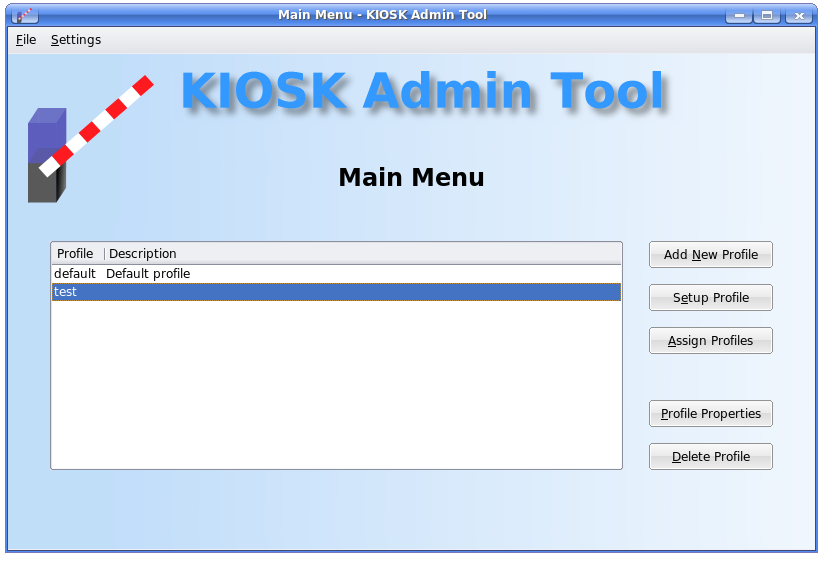
\includegraphics[width=8.5cm]{obrazky/KioskToolKDE3/uvodni_obrazovka.png}
    \caption{Úvodní obrazovka programu}
    \label{fig:kt3_uvodni}
\end{figure}
Úvodní obrazovka \ref{fig:kt3_uvodni} ukazuje seznam profilů s jejich popisem,
lištu s menu a tlačítka pro manipulaci s profily. Velmi chybí možnost zkopírovat
již existující profil.

\begin{figure}[h]
    \centering
    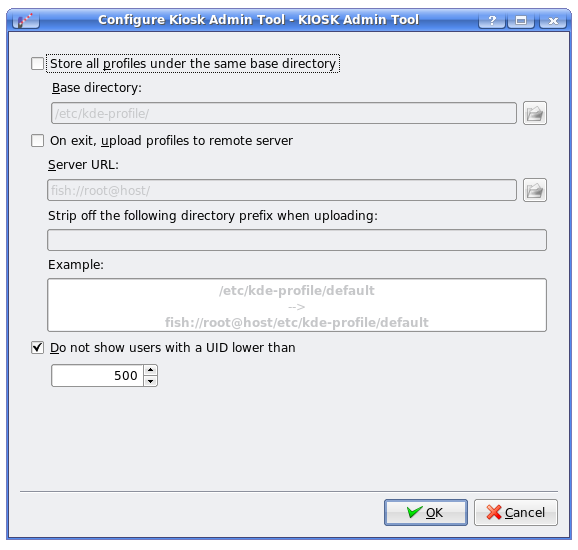
\includegraphics[width=8.5cm]{obrazky/KioskToolKDE3/nastaveni.png}
    \caption{Dialogové okno s nastavením}
    \label{fig:kt3_nastaveni}
\end{figure}
Mezi nastavení programu \ref{fig:kt3_nastaveni} patří také možnost automaticky
uložit profily na vzdálený serber.

\begin{figure}[h]
    \centering
    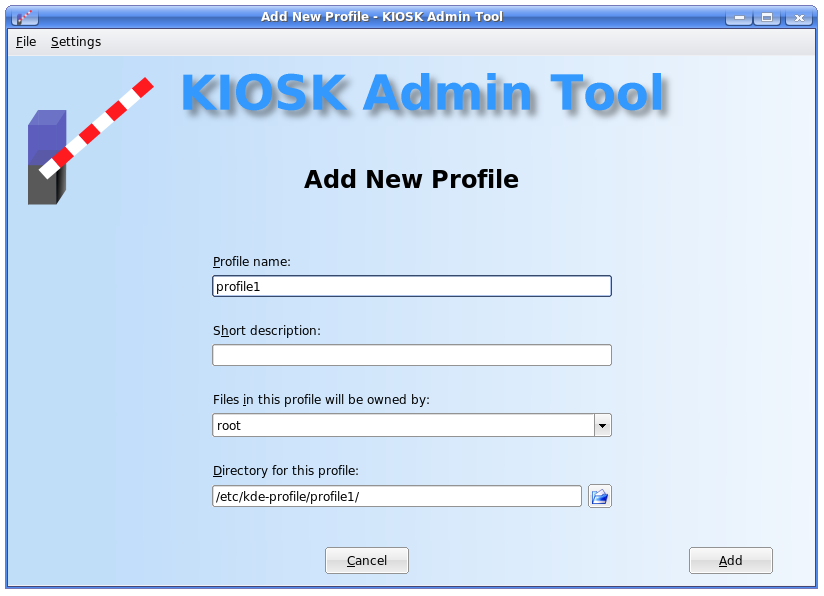
\includegraphics[width=8.5cm]{obrazky/KioskToolKDE3/novy_profil.png}
    \caption{Dialog pro vytvoření nového profilu}
    \label{fig:kt3_novyprofil}
\end{figure}
Dialog pro vytvoření nového profilu \ref{fig:kt3_novyprofil} je poměrně
jednoduchý. Umožňuje nastavit název a popis profilu a dále který uživatel bude
vlastnit složku s profilem (bude mít přístup pro zápis) a kde bude profil
uložen.

\begin{figure}[h]
    \centering
    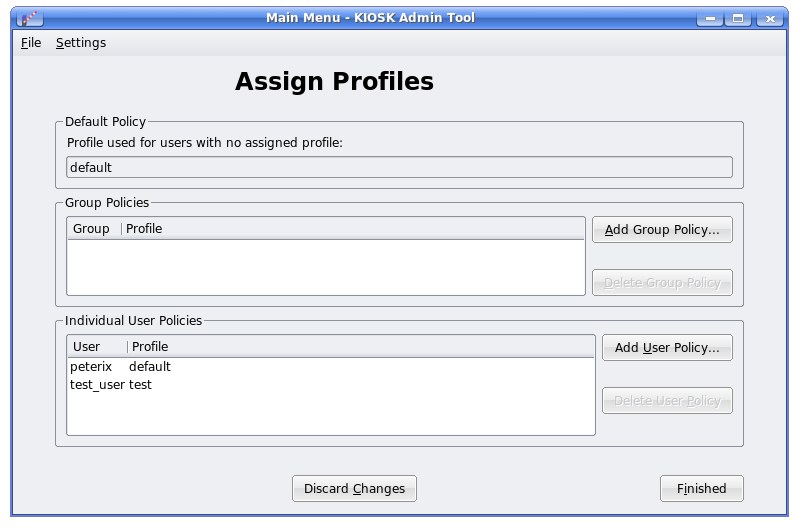
\includegraphics[width=8.5cm]{obrazky/KioskToolKDE3/prirazeni_profilu.png}
    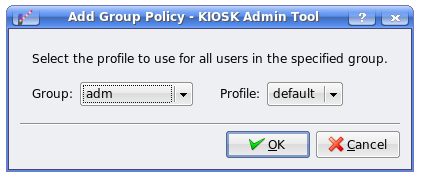
\includegraphics[width=8.5cm]{obrazky/KioskToolKDE3/prirazeni_profilu_skupine.png}
    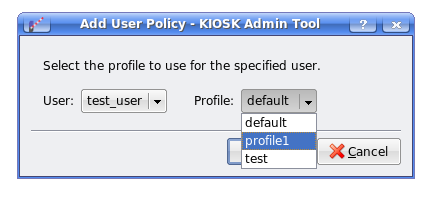
\includegraphics[width=8.5cm]{obrazky/KioskToolKDE3/prirazeni_profilu_uzivateli.png}
    \caption{Dialogy pro přiřazení profilů}
    \label{fig:kt3_prirazeni}
\end{figure}
Při pohledu na obrazovku a dialogy pro přiřazení Kiosk profilů skupinám
a uživatelům je nutné si připomenout, že když má uživatel přířazen svůj vlastní
profil, nevztahují se na něj profily pro skupiny kterých je členem. To program
nijak nezvýrazňuje. Bylo by dobré, kdyby poskytoval nějaký pohled, který by
ukazoval všechny profily efektivní pro uživatele.

\begin{figure}[h]
    \centering
    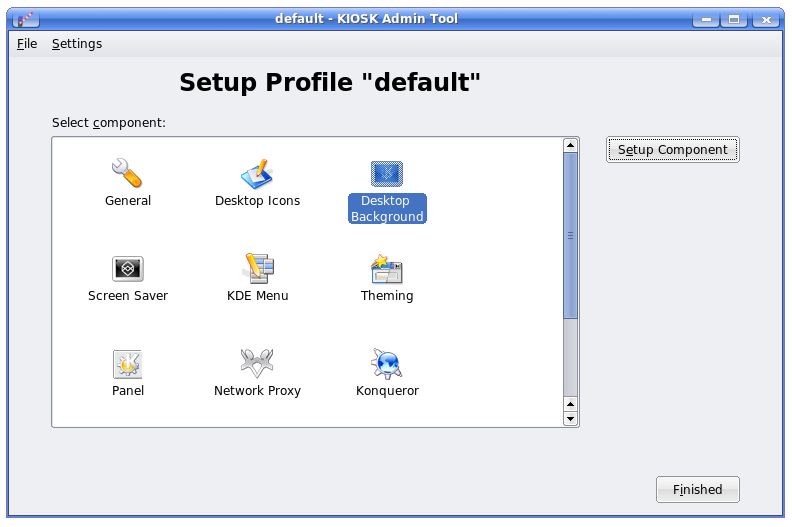
\includegraphics[width=8.5cm]{obrazky/KioskToolKDE3/seznam_komponent.png}
    \caption{Dialog s nastavením profilu}
    \label{fig:kt3_nast_prof}
\end{figure}
Dialog pru úpravu profilu \ref{fig:kt3_nast_prof} je mohem zajímavější. Je možné
z něj spouštět KCM moduly a jiné části systému KDE a tak docílit toho,
že KioskTool může využít již existující funkcionalitu. Není proto nutné znovu
'vymýšlet kolo' a uživatel pro nastavení Kiosk profilů používá stejné nástroje
jako pro normální nastavení. Tato původní verze nástroje KioskTool definuje
všechny moduly a jejich vlastnosti v jednom velkém XML souboru.

\begin{figure}[h]
    \centering
    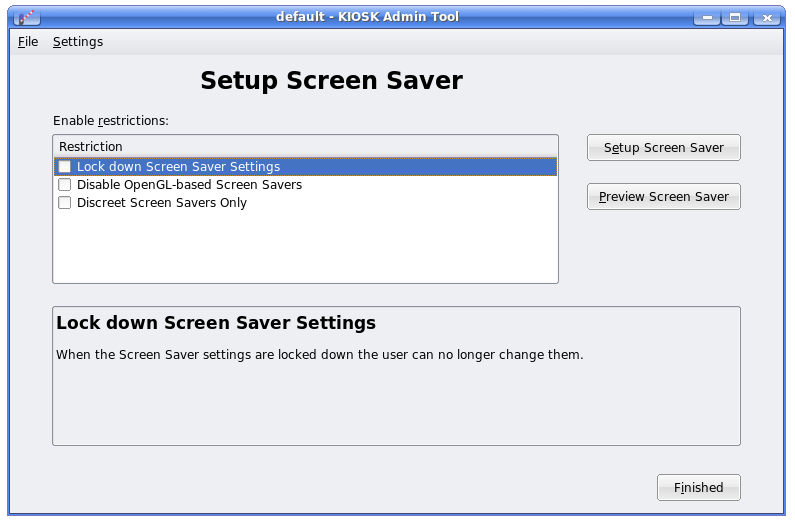
\includegraphics[width=8.5cm]{obrazky/KioskToolKDE3/ukazka_komponenty.png}
    \caption{Dialog jedné komponenty nástroje}
    \label{fig:kt3_nast_komp}
\end{figure}
Na obrázku \ref{fig:kt3_nast_komp} je vidět jak taková komponenta vypadá
v akci. Uživatel může uzamčít obrázek na pozadí plochy a ukázat si náhled tohoto
obrázku (náhled ve smyslu, že se pozadí plochy dočasně zamění). Zde by asi bylo
lepší místo náhledu otvírat KCM modul pro nastavení plochy a případně nějaký
režim pro rozvržení plasmoidů  na ní. Zejména kvůli tomu, že v KDE4 je původně %!REF! plasma
jednoduchá plocha nahrazena plochou plasma a tam je mnohem více věcí
k nastavování.

I při krátké době nutné na seznámení s nástrojem (KioskTool 1.0 v Kubuntu 9.04)
jsem narazil na fatální chyby, kdy se bez zjevného důvodu zhroutil. Nebude tedy
možné se spolehnout na korektnost kódu.

\begin{figure}[h]
    \centering
    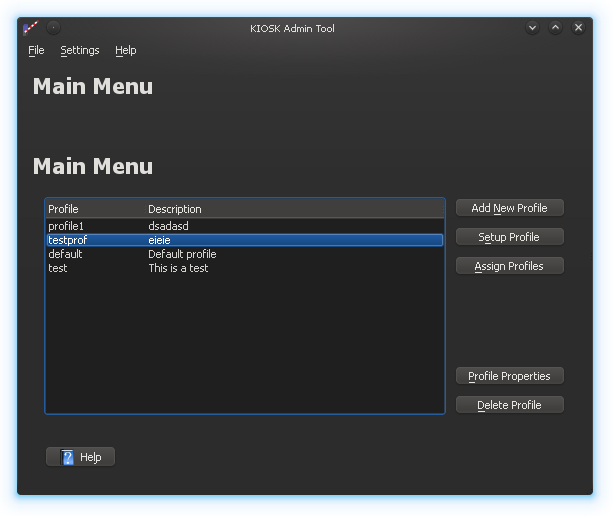
\includegraphics[width=8.5cm]{obrazky/KioskToolKDE4/kiosktool_kde4.png}
    \caption{=U}
    \label{fig:kt4_uvod}
\end{figure}

Port nástroje do KDE4 \ref{fig:kt4_uvod} již existuje, i když je značně
nedokončený.  %Ref: Kdo portoval, kde lze najít, proč toho nechal tak brzo?
Původní nastavení pomocí velkého XML souboru bylo odstraněno a nahrazeno mnoha
menšími .ini soubory. To má za účel umožnit ostatím autorům napsat pro jejich
aplikace moduly do nástroje KioskTool. Nástroj ztratil většinu svých modulů,
schopnost spouštět KCM moduly a náhledy, své pěkné (i když zbytečné) obrázkové
vzezření a získal několik dalších chyb. Zdá se ale, že na něm stále někdo
pracuje. %ref: Luboš Luňák?

\section{PolicyKit}
\begin{figure}[h]
    % toto je překreslené z man stránky. Jak citovat?
    \centering
    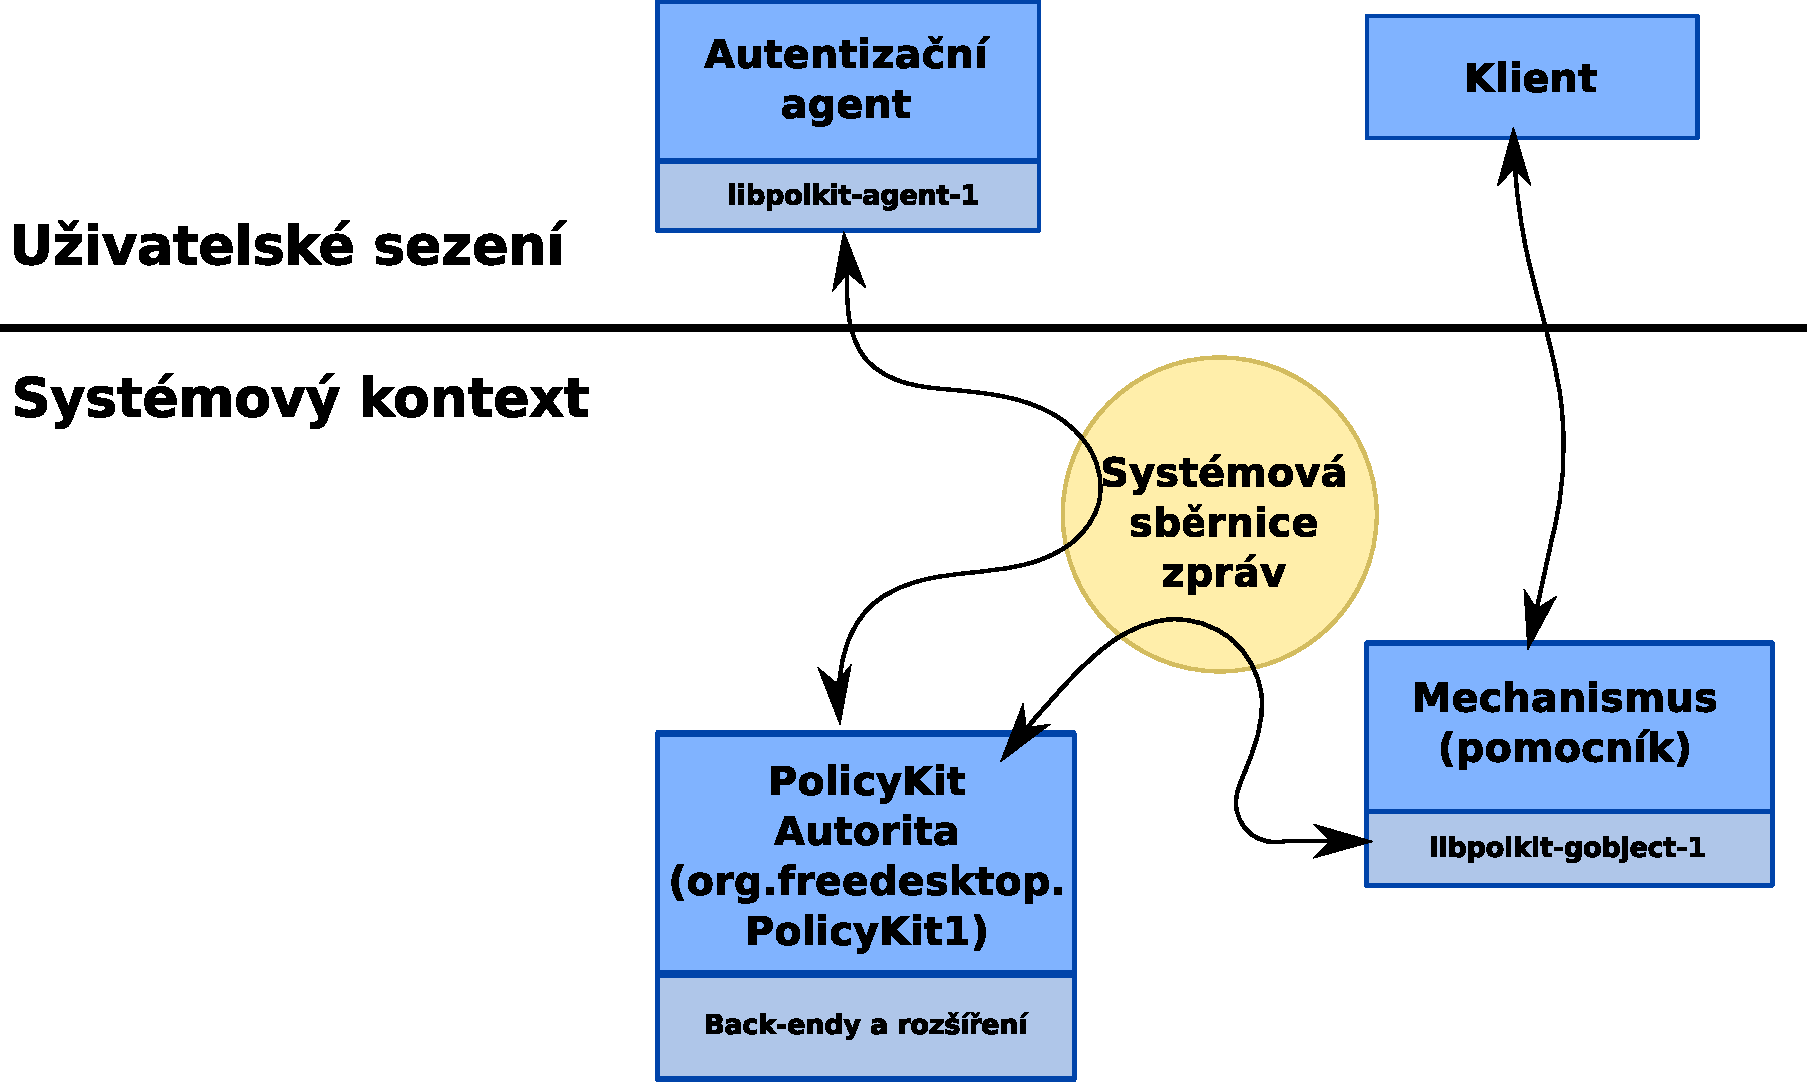
\includegraphics[width=12cm]{obrazky/polkit-architecture-vector-cz.pdf}
    \caption{Architektura systému PolicyKit}
    \label{fig:polkit_arch}
\end{figure}

PolicyKit (přejmenován na polkit), je systém umožňující autentizovat uživatele,
autorizovat akce těchto uživatelů a pomocí tzv. mechanismů tyto akce také
provádět. Je to systém velmi modulární a přenechává implementaci mnoha těchto 
funkcí zásuvným modulům a programům které jej využívají. Pro každý typ rozšíření
PolicyKitu existuje knihovna. Jednotlivé komponenty pak spolu komunikují pomocí
IPC mechanismu DBUS (ať už přímo nebo prostřednictvím knihoven).

Mezi nejzákladnější části tohoto systému patří démon polkitd, implementující
část PolicyKit Authority. Ta se stará o uložení databáze možných akcí
a povolení a slouží jako centrální prvek celého systému.

Další částí, implementovanou prostředími jako je Gnome nebo KDE je tzv.
autentizační agent. To je program, který například uživateli zobrazí okno pro
zadání hesla, pokud je potřeba ověřit jeho totožnost. Pro samotné ověření je
možné použít pomocný program běžící se superuživatslkými právy a používající
k ověření systém jako je PAM. To ale není striktně vyžadováno. Lze i jen
zobrazit obyčejné okno s dotazem typu Ano/Ne.% REF! REF! REF!

Třetí komponentou je 'mechanismus' nebo 'pomocník' -- zde se jedná o službu pro
vykonání privilegovaných akcí místo uživatele, který o provedení akce žádá.
Čtvrtou a poslední komponentou je klient -- program, který využívá služeb
systému PolicyKit.
% REF IPC, REF DBUS!

Průběh akcí v systému pro volání funkce pomocníka může vypadat napříklat takto:
\begin{itemize}
\item Uživatel se přihlásí, je nastartováno sezení KDE a s ním i autentizační
agent
\item Autentizační agent se registruje u PolicyKit autority
\item Uživatel spustí program, který využívá služeb PolicyKitu
\item Program zavolá funkci pomocníka přes systém DBUS
\item DBUS démon nastartuje program pomocníka, pokud již neběží (pomocník musí
být v systému DBUS registrován)
\item Spuštěný pomocník se zeptá PolicyKit autority, jestli je volaná akce
autorizována
\item PK autorita zkontroluje, jestli je již tato akce autorizována (autorizace
může mít například platnost pro celé sezení). Pokud není zatím autorizována,
zjistí jakým způsobem se má dosáhnout autorizace.
\item Pokud je to nutné, zavolá PK autorita autentizačního agenta. Zobrazí se
například okno, kde má uživatel zadat své login údaje. Je možné ověřovat buď
pouze identitu uživatele, kdy stačí, že se přihlásí pod vlastním účtem,
nebo je možné vyžadovat přihlášení účtu se superuživatslkými právy.
\item Uživatel se přihlásí (záleží na tom jaký mechanismus k tomu agent
používá).
\item Agent oznámí autoritě jestli byla autentizace úspěšná.
\item Autorita vrací výsledek autorizace a uloží si ho do cache po dobu její
platnosti.
\item Pokud byl proces autorizacu úspěšný, pomocník provede požadovanou akci.
\item V tomto bodě může pomocník notifikovat program o výsledku akce.
\end{itemize}

Toto samozřejmně není jedniný možný průběh. Vše záleží na implementaci
jednotlivých komponent. Jak jsem již uvedl, PolicyKit je velmi modulární systém
a většinu jeho částí lze nahradit nebo rozšířit.

Nad PolicyKitem je postavena knihovna polkit-qt. Poskytuje v zásadě stejné
funkce jako PolicyKit a lépe je integruje do prostředí knihoven QT. % REF!

Polkit-kde je nadstavbou nad knihovnou polkit-qt, která implementuje autentizačí
agent pro prostředí KDE a KCM modul pro úpravu akcí povolených pro uživatele
a skupiny.

Zatím jediným způsobem uložení povolených akcí v PolicyKitu je tzv. lokální
autorita. Je to výchozí implementace PolicyKit Autority a využívá lokálně
uložených textových souborů s příponou .pkla. Efektivní seznam povolených akcí
se získá služením těchto souborů. Je tedy možné mít například jeden soubor
s výchozím nastavením instalovaný z distribučního balíčku a druhý s lokálním
nastavením, vytvořený administrátorem.

\begin{figure}[h]
    \centering
    \begin{verbatim}
                   /var/lib/polkit-1
                   └── localauthority
                       ├── 10-vendor.d
                       │   └── 10-desktop-policy.pkla
                       ├── 20-org.d
                       ├── 30-site.d
                       ├── 50-local.d
                       ├── 55-org.my.company.d
                       │   └── 10-org.my.company.product.pkla
                       └── 90-mandatory.d

                   /etc/polkit-1
                   └── localauthority
                       ├── 10-vendor.d
                       │   └── 01-some-changes-from-a-subvendor.pkla
                       ├── 20-org.d
                       ├── 30-site.d
                       ├── 50-local.d
                       ├── 55-org.my.company.d
                       │   └── 10-org.my.company.product.pkla
                       └── 90-mandatory.d
    \end{verbatim}
    \caption{Struktura složek pro PolicyKit Local Authority s několika .pkla soubory}
    \label{fig:pkit_la}
\end{figure}

Local Authority pro ně zavádí poměrně propracovanou strukturu \ref{fig:pkit_la}.
Pořadí načítání je určeno lexikografickým řazením složek a souborů v nich.
Pokud je stejně pojmenovaný soubor v obou umístěních (ve /var/lib/ i /etc/),
nejdříve se zpracuje ten ve /var/.
%REF: cite man stránka pklocalauthority
Ve struktuře \ref{fig:pkit_la} by pořadí zpracování vypadalo takto:
\begin{itemize}
\item 10-desktop-policy.pkla
\item 01-some-changes-from-a-subvendor.pkla
\item 10-org.my.company.product.pkla (z /var)
\item 10-org.my.company.product.pkla (z /etc)
\end{itemize}

%TODO: jak vypadá .pkla soubor, jak se zpracovává

\section{KAuth}
KAuth je nové rozhraní pro autorizaci v KDE. Je postaveno na již existujících 
rozhraních v operačních systémech. V OS na bázi Linuxu je to zpravidla
PolicyKit, v OSX pak framework Authorization Services. Podporu pro nová rozhraní
je možné přidat pomocí zásuvných modulů.

Pomocí KAuthu je možné autorizovat akce uživatele. Zásuvný modul se stará
o veškeré ověřování akcí. Z pohledu PolicyKitu je zde aplikace používající
KAuth v roli klienta.
Další funkce poskytovaná KAuthem je vytvořit pokud možno co nejjednodušší
program, který pak bude v odpověď na autorizovanou akci spuštěn příslušným
autorizačním rozhraním. Takovýto program se nazývá KAuth pomocník (helper).
Pomocník a aplikace která ho využívá mohou do jisté míry komunikovat oběma směry
a je také možné sledovat průběh dlouho trvající akce uvnitř pomocníka. KAuth
pomocník je rozšířením PolicyKit pomocníka o tyto zjednodušené komunikační
funkce.

Další službou KAuthu je registrace pomocníků a akcí v jeho jednotlivých
zásuvných modulech. Uživatel KAuthu tedy specifikuje, jaké akce a pomocníky chce
použít a při kompilaci budou převedeny do formy srozumitelné pro jeho zásuvné
moduly.

KAuth nepodporuje provádění změn v nich po kompilaci. Také neumožňuje měnit
autorizované uživatele a skupiny pro akce -- to je zcela přenecháno systémům pro
autorizaci, které využívá. V případě PolicyKitu je toto nastavní realizováno
v KControl modulu, který používá přímo knihovnu polkit-qt. Další nepodporovanou
částí je jakákoliv idea bezpečnostních profilů přiřazovaných uživatelům
a skupinám. Nic takového konec konců není ani v PolicyKitu, který byl KAuthu
modelem. Toto jsou celkem závažné nedostatky, které budu muset nějak vyřešit.

\subsection{PolicyKit KControl modul (KCM)}
\chapter{Změny v~KAuthorized, KAuth}
První skutečnou částí projektu je zjistit jak nejlépe integrovat systém KAuth do
rozhraní KAuthorized. Toto není triviální úkol a nějakou dobu mi trvalo, než
jsem přišel na to, jak toho docílit. Začnu popisem dvou variant, které jsem
musel pro závažné nedostatky zavrhnout (postupně jak jsem analyzoval jednotlivé 
využitelné technologie). Třetí variantu, kterou budu implementovat, popisuji
ve třetí sekci kapitoly.
\section{Slepé uličky}
Můj první a také nejjednodušší nápac byl vytvřit statický .actions soubor
a integrace KAuth přímo do KAuthorized. V zásadě by toto mohlo fungovat a je
to částí řešení.

Prvním problémem je, že neexistuje definitivní seznam možných restrikcí akcí
a zdrojů v Kiosk profilech. Toto by šlo řešit tak, že každý program KDE by tyto
své akce a zdroje specifikoval v .actions souboru k tomu určeném a zahrnul by
jeho překlad do KAuthem podporovaných systémů do svého sestavení. To ovšem
vylučuje jakoukoliv možnost stejné úrovně podpory pro aplikace, které by takto
akce nespecifikovaly.

Druhým problémem je neexistence možnosti nastavit autorizované akce pro
uživatele a skupiny pomocí KAuthu. Nejen že nejdou nastavit, KAuth navíc nemá
ani žádné ponětí o něčem, co by alespoň vzdáleně připomínalo způsob jakým
se aplikují Kiosk profily. V případě použití PolicyKitu tyto vcelku základní
funkce nemé ve formě knihovny žádná vrstva - PolicyKit, polkit-qt, polkit-kde
ani KAuth.

Řešení tedy musí vypadat velmi odlišně.

Druhý nápad byl takovýto: když KAuth nepodporuje nic z toho, co by korektní
implementace vyžadovala, bude nutné to nějak obejít, a to co nejjednodušším
způsobem, aby zbytečně nedošlo k zavlečení chyb.

Takovým možným řešením je jednoduše se vzdát toho, že budeme mapovat akce mezi
Kioskem a KAuthem jedna ku jedné. Mělo by být přece možné umístit do KAuth
pomocníka instanci KConfigu, která načte požadovaný Kiosk profil a bude přes
systém DBUS umožovat dotazování se na jednotlivé hodnoty v nich. Bylo by také
možné tyto hodnoty měnit. V podstatě by to byl stále pouze KConfig, jen obalen
v pomocníkovi.

Problémy tohoto řešení nemusejí být zcela zjevné, pokusím se je ale popsat.
Za prvé -- nezíská se tím vůbec žádná výhoda z pohledu bezpečnosti. Kiosk
profily musejí stále zůstat čitelné pro všechny uživatele, jinak by se
nenačetly při spuštění programů nemohly načíst a tím by byly zcela neefektivní.
Odpadá tak výhoda KAuthu, kde jak seznam restrikcí, tak jaké restrikce pro koho
platí může být skryt před uživateli. Například při použití PolicyKit Local
Authority je možné nastavit všechny soubory čitelné jenom superuživatelem.

Za druhé -- KAuth pomocníci mají omezenou životnost. Pokud nejsou využíváni po
dobu deseti vteřin, jsou ukončeni. Znamená to znovu načíst celý KConfig objekt.
I když je toto načítání vysoce optimalizováno, stále je vcelku zbytečné načítat
celou konfiguraci dvakrát - jednou v programu, který by volal KAuthorized
a podruhé v KAuth pomocníkovi. Sdílet zde jeden objekt například umístěním
do sdílené paměti by byl holý nesmysl, takže se taková věc ještě více prodraží
-- použijeme až dvakrát více paměti.
Toto všechno by šlo obejít, ale výsledek by neměl žádný smysl a jeho šance na
integraci do KDE by byla prakticky nulová.

Dalším problémem je, že takto nezískáme ani jiné výhody KAuthu. Za zmínku stojí
například integrace s instalovaným systémem správy autorizací. Jediné co přibude
je jeden program a několik málo akcí které podporuje.

Je tu ještě jeden problém -- KAuth podporuje použití pomocníků pouze
v kombinaci se systéme PolicyKit a DBUS. Uživatelé Windows a OSX mají smůlu.
Tomu se asi nevyhneme.

Je vidět, že ani tudy cesta nevede. Jak tedy postupovat když se zadání zdá být
nesplnitelné?

\section{Možné řešení}
Řešení nebude až tak pěkné jak by mohlo být, kdyby KAuth podporoval zápis
autorizací jakožto knihovní funkci.

Začneme se specifikacemi akcí u jednotlivých programů. Definovat je centrálně
tak, aby se instalovaly spolu s KioskTool nástrojem by nevedlo k ničemu dobrému
(někdo by je musel udržovat). Každý softwarový balík a program v KDE tedy bude
muset specifikovat své akce a zdroje ve formě srozumitelné pro KAuth - .actions
souborem. Jedná se o zdroj dat specifický pro aplikaci a jakékoliv akce, které
implementuje nad rámec standardních akcí obsažených v KDE. Použití KAuth
by nemělo být povinné a mělo by být zachováno chování rozhraní KAuthorized pokud
možno tak, aby se z pohledu aplikací nic nezměnilo.

Dále je potřeba implementovat konvertor Kiosk profilů na nastavení lokálního
systému pro autorizaci. Zde se budu muset držet PolicyKitu, protože jediný další
podporovaný systém je Authorization Services v operačním systému Apple OSX.
Hardware potřebný pro legální provoz OSX bohužel nemám.
Takovýto konvertor by měl umět běžet jak KAuth pomocník i jako samostatný
program spustitelný superuživatelem z příkazové řádky. Konverze z Kiosk profilů
bude jednosměrná, bude používat polkit-qt pro získání seznamu podporovaných
restrikcí a bude produkovat soubory .pkla, použitelné jen a pouze v PolicyKit
Local Authority. Konvertor by mělo být možné, až bude stabilní, integrovat
do KAuthu nebo balíku policykit-kde.

Omezení konvertoru je zjevné -- pokud bude použita jiná autorita než PolicyKit
Local Authority, konverze s ní nebude fungovat. Vzhledem k tomu, že tato
autorita je výchozí, předpokládám, že bude k dispozici.

V konvertoru je nutné zohlednit to, že postup aplikace profilů v Kiosku je jiný
než postup ověření autorizace v PolicyKitu. Musí se 'nasimulovat' Kiosk a jeho
zvláštnosti, aby se nezměnilo chování KAuthorized.

Integrace KAuth do KAuthorized by měla být triviální záležitost -- otázka
několika volání funkcí KAuth. Musí se počítat s tím, že KAuth nemusí být
funkční (je v nové verzi použité pro tuto práci stále ještě nestabilní) nebo že
konvertor zatím nikdy nebyl spuštěn a v těchto případech použít normální
nastavení Kiosk profilu přes KConfig.

\section{Implementace konvertoru}


\chapter{Úpravy nátroje KioskTool}
\section{Uživatelské rozhraní}
\section{Integrace KAuth}
\section{Spouštění KCM modulů}
\chapter{Další možný postup a návrh systematických změn v KDE}
\chapter{Testování a začlenění do KDE}
\chapter{Závěr}
\cite{fitWeb}
%=========================================================================
